\famichapter{System Architecture and Design}{This chapter describes the logical
architecture of FamiPet, the request lifecycle, the deployment layout, and the
responsibility of each component.}{ch:arch}

\section{Architecture Style}

FamiPet is a client--server application whose backend is a \emph{modular
monolith}: one Express process exposes all sixteen route modules, and all
business logic, validation, and persistence live in that process against a single
MongoDB store. There are no microservices, no message broker, and no background
workers. This architecture was chosen because the functional requirements are
interdependent (appointments create reminders and notifications; adoption
approval updates the pet and notifies the applicant) and the data is shared, so a
single transaction context keeps the flows simple, consistent, and testable.

Figure~\ref{fig:layered} shows the layered structure of the backend as it is
implemented. The presentation boundary is the HTTP API consumed by the web
client. Gateway middleware sets the security and parsing context. The routing
layer maps the sixteen route modules, and access-control middleware
(\texttt{protect}, \texttt{adminOnly}, \texttt{upload}) enforces identity,
roles, and file constraints. The controller layer implements the business logic.
The data layer maps the 13 Mongoose models to MongoDB collections. Two external
boundaries are drawn: e-mail and AI.

\begin{figure}[htbp]
    \centering
    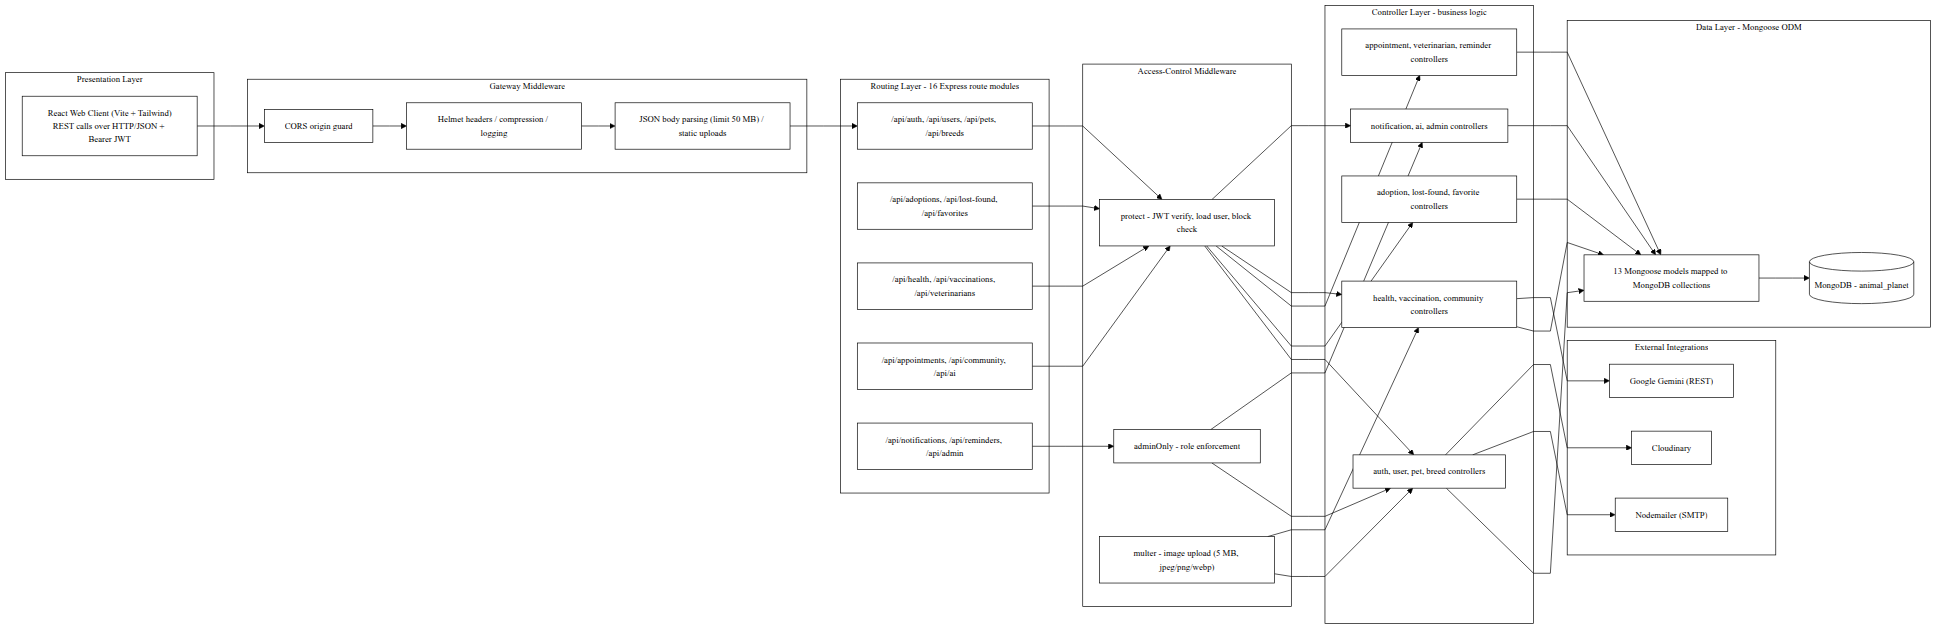
\includegraphics[width=\textwidth]{figures/04-layered-arch.png}
    \caption{Layered architecture of the FamiPet backend.}
    \label{fig:layered}
\end{figure}

The layered diagram reflects the actual module boundaries of the repository.
Cross-cutting concerns (CORS, helmet, compression, JSON parsing) run before any
route module. The \texttt{protect} middleware runs on every protected route, the
\texttt{adminOnly} middleware on administrative routes, and the
Multer~\cite{multer} upload
middleware only on routes that accept images.

\section{Module Responsibilities}

The table below lists the sixteen Express route modules and the central
responsibilities of their controllers.

\begin{center}
\begin{longtable}{@{}p{3.6cm}p{11.0cm}@{}}
\caption{Backend route modules and responsibilities.}
\label{tab:modules}\\
\toprule
\textbf{Route module} & \textbf{Responsibility} \\
\midrule
\path{/api/auth} & Register, verify and resend e-mail verification, login,
forgot/reset password, current user, profile update, password change. \\
\path{/api/users} & Public user lookup, favorites toggle, avatar upload. \\
\path{/api/pets} & Public pet listing, featured pets, own pets, pet CRUD with
owner enforcement, QR generation. \\
\path{/api/breeds} & Public breed catalogue; admin create/update/delete. \\
\path{/api/adoptions} & Adoption applications, own applications, admin listing
and status updates with pet transition and notification. \\
\path{/api/lost-found} & Public reports, owner CRUD, admin status updates and
deletion. \\
\path{/api/health} & Owner-scoped health records per pet. \\
\path{/api/vaccinations} & Owner-scoped vaccination records and upcoming list. \\
\path{/api/favorites} & Owner-scoped favourite pets (unique user--pet pairs). \\
\path{/api/veterinarians} & Public directory; admin CRUD. \\
\path{/api/appointments} & Booking with slot conflict check, auto-notification
and auto-reminder, reschedule and cancel with reminder sync. \\
\path{/api/community} & Public posts, owner CRUD, likes, comments; admin
moderation. \\
\path{/api/ai} & \texttt{/ask} (PetGPT over Gemini with fallback) and
\texttt{/advice} (rule-based per-pet advice). \\
\path{/api/notifications} & Owner-scoped notification read, unread, mark
read/all-read, delete. \\
\path{/api/reminders} & Owner-scoped reminders CRUD and completion. \\
\path{/api/admin} & Dashboard statistics, user/pet/lost-found/community
administration. \\
\bottomrule
\end{longtable}
\end{center}

\section{Request Lifecycle}

Figure~\ref{fig:lifecycle} shows the lifecycle of a protected request, using the
example of an authenticated controller that owns a resource. The sequence is
identical for every protected subsystem; the ownership predicate is the only
part that varies (see Chapter~\ref{ch:auth}).

\begin{figure}[htbp]
    \centering
    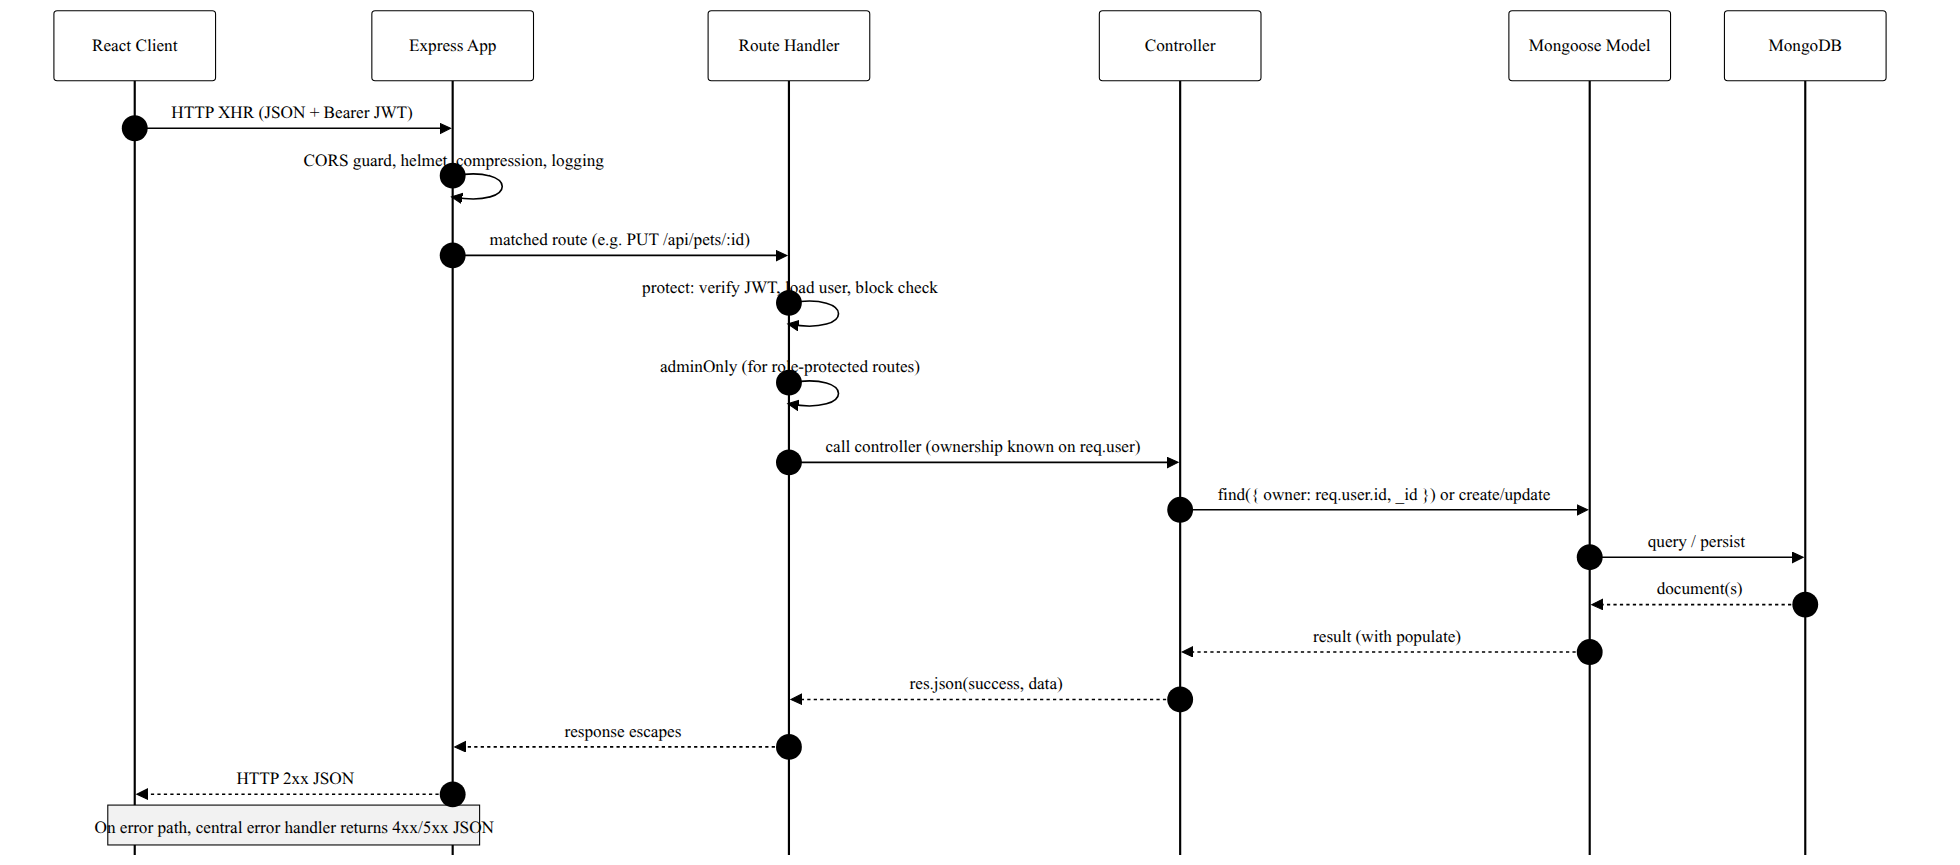
\includegraphics[width=\textwidth]{figures/06-request-lifecycle.png}
    \caption{Lifecycle of a protected request through the backend.}
    \label{fig:lifecycle}
\end{figure}

Once the token is verified and the user is loaded, owner-scoped queries bind the
resource to \texttt{req.user.\_id}: for example, appointments are queried with
\texttt{\{user: req.user.\_id\}}, health records and vaccinations the same way,
and pet operations compare \texttt{pet.owner} to \texttt{req.user.id}. This
binding is what makes user isolation enforceable without trusting any
client-supplied identifier.

\section{Deployment}

Figure~\ref{fig:deploy} shows the deployment layout used during the project. The
backend process and the frontend are served on different ports; the database
runs as a separate service, optionally with local tooling (Compass) for
inspection. The backend also serves the \texttt{uploads} directory statically so
uploaded images resolve from the API. Credentials for the optional external
image-hosting platform Cloudinary~\cite{cloudinary} are declared in the
configuration but the current implementation stores uploads locally on disk.

\begin{figure}[htbp]
    \centering
    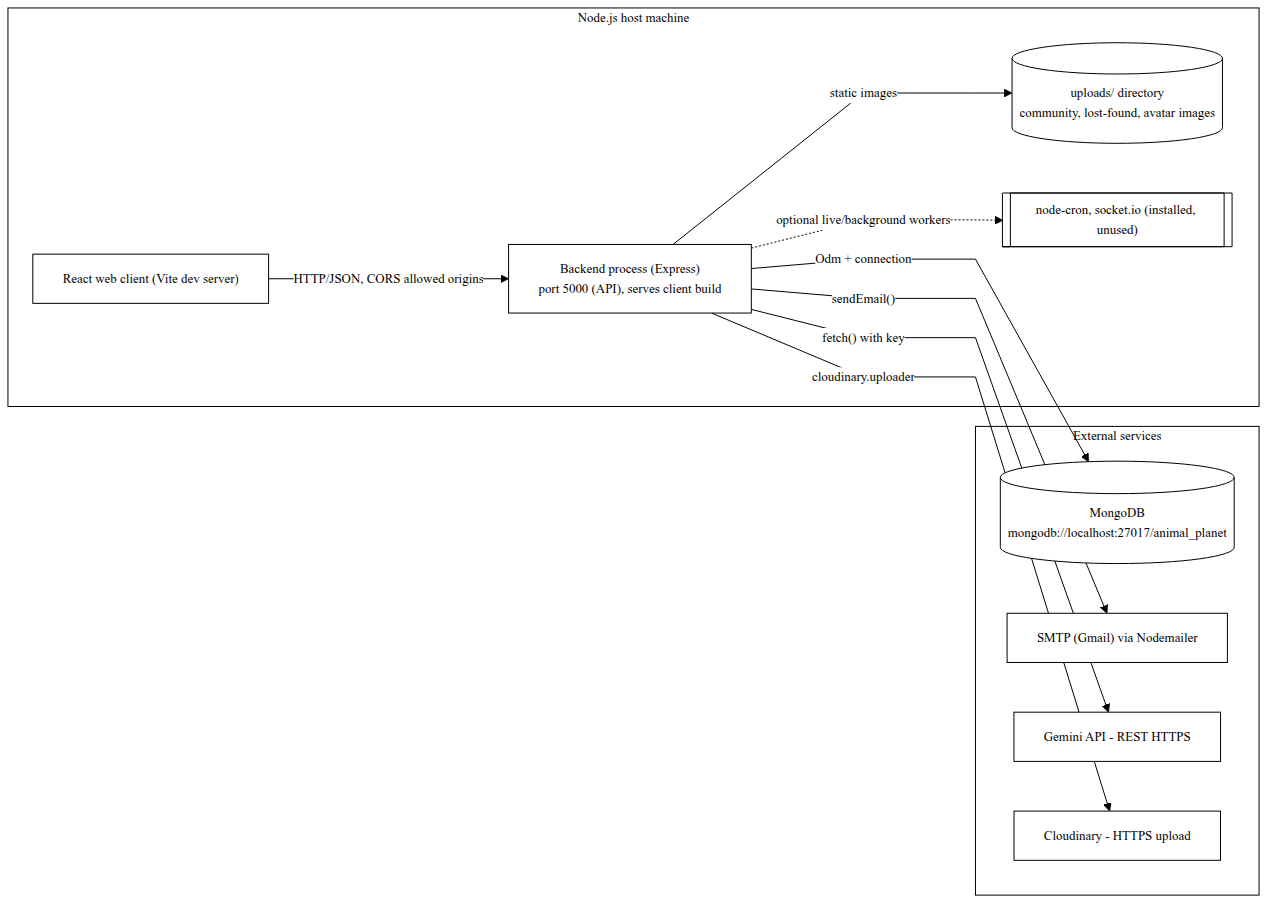
\includegraphics[width=\textwidth]{figures/07-deployment.png}
    \caption{Deployment layout of FamiPet.}
    \label{fig:deploy}
\end{figure}

The server binds to the environment-configured port (5000 by default). The
client origin is taken from \texttt{CLIENT\_URL} (5000-series Live Server/Vite by
default) and is also used to fall back to a locally served page for the
verify-email and reset-password routes. MongoDB connects through
\path{MONGODB\_URI}, defaulting to
\path{mongodb://localhost:27017/animal\_planet}.